\chapter{Synopsis}

\section{Concepts}

\subsection{Concept du Google Cardboard}

\begin{figure}[h!]
  \centering
  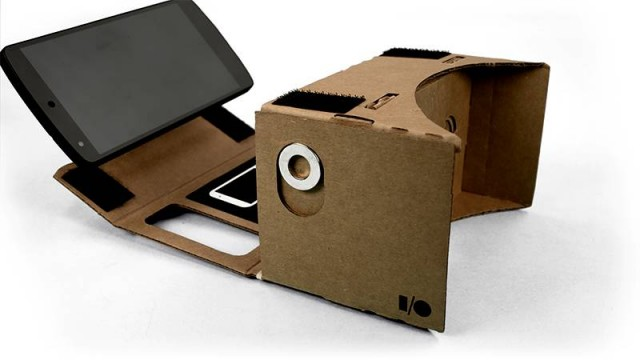
\includegraphics[width=0.7\textwidth]{res/img/cardboard1.jpg}
  \caption{Google Cardboard avec un téléphone}
\end{figure}

Juin 2014, Google dévoile Cardboard lors de sa conférence annuelle. Cet appareil en carton et plastique (lentilles) permet, à l'aide d'un smartphone que l'on insère dedans, de plonger l'utilisateur dans un environnement 3D virtuel. L'outil se présente sous la forme d'une boîte avec deux lentilles grossissantes placées entre les yeux et le téléphone disposé horizontalement. Un \og{}bouton\fg{} magnétique (aimant) offre une interaction très simpliste à l'utilisateur, disposé sur le côté gauche de l'appareil.

\subsection{Possibiltés}

\noindent Les Cardboards nous offrent principalement 4 types de projets potentiels :

\begin{itemize}
  \item Utiliser Google Maps (et donc Google StreetView) pour plonger l'utilisateur dans une planète Terre virtuelle (construite à base de photos)
  \item Créer un environnement 3D virtuel avec OpenGL ou Unity
  \item Afficher l'environnement de l'utilisateur grâce la caméra dorsale du téléphone
  \item Afficher des photos sphères (photos prises à 360° avec la caméra)
\end{itemize}
Nous avons choisi de nous orienter vers \textbf{la création d'un environnement 3D virtuel avec Unity}.

\subsection{Concept de notre projet}

\textbf{Il s'agira d'un jeu.} L'utilisateur, au départ du jeu, sera plongé dans un \textbf{labyrinthe 3D}. Le but du jeu sera simple : \textbf{sortir du labyrinthe}. Le bouton (aimant) permettra alternativement de placer le joueur en déplacement ou à l'arrêt, le choix de la direction de déplacement se faisant \og{}en réel\fg{} (le joueur devra se tourner sur lui-même pour aller à gauche ou à droite dans le jeu, cela étant possible grâce au giroscope du téléphone).

\section{Public-cible}

Ce projet s'adresse à tout type d'utilisateur disposant d'un smartphone assez récent pour être utilisé avec Google Cardboard. Il n'y pas pas de contre-indication particulière à l'usage des Cardboard. Toute personne
voulant tester la réalité virtuelle est susceptible de jouer, quelque soit son âge.

\section{Objectif}

\subsection{Objectif principal}

Notre projet consiste à créer un labyrinthe 3D dans lequel l'utilisateur serait placé, le but pour lui étant d'en sortir. Les déplacements possibles seront \og{}avancer\fg{}, \og{}tourner à droite\fg{} ou \og{}à gauche\fg{}. L'utilisateur aura également la possibilité de s'arrêter/d'avancer en utilisant l'aimant des Cardboards. Pour tourner, il suffira à l'utilisateur de réellement tourner sur lui même. Ce mouvement sera détecté grâce au gyroscope du téléphone utilisé et nous permettra de changer la direction du joueur dans le labyrinthe.

\subsection{Objectifs complémentaires}\label{sub:objectifs_complementaires}

Suivant le temps qu'il nous faudra pour prendre en main Unity (l'outil utilisé pour créer un environnement 3D), d'autres fonctionnalités pourront être envisagées telles que :
\begin{itemize}
  \item Rajouter une ambiance sonore
  \item Génération aléatoire du labyrinthe ou création de plusieurs labyrinthes, et non un seul
  \item Création d'un \textit{Pacman-like} (avec d'autres joueurs contrôlés par le téléphone -- intelligence artificielle -- poursuivants le joueur)
  \item Durée de jeu limite dans laquelle le joueur doit trouver la sortie
  \item Possibilité de jouer à plusieurs (avec plusieurs Cardboards)
  \item Possibilité d'obtenir des bonus en ramassant des objets
  \item Possibilité de plonger l'utilisateur dans le noir pendant un court instant
\end{itemize}

\subsection{Résumé}
Ce projet fait donc appel à trois types d'intéractions : \textbf{visuelles, sonores et gestuelles}. L'objectif pour nous est d'offrir une expérience immersive à l'utilisateur. Puisqu'il s'agit d'un jeu non éducatif, aucun connaissance particulière n'est apportée au joueur, seuls ses sens sont mis à l'épreuve ! De la peur et du stress pourront éventuellement naître, notamment si nous parvenons à insérer d'autres joueurs ou mettre un temps limite.

\begin{figure}[h!]
  \centering
  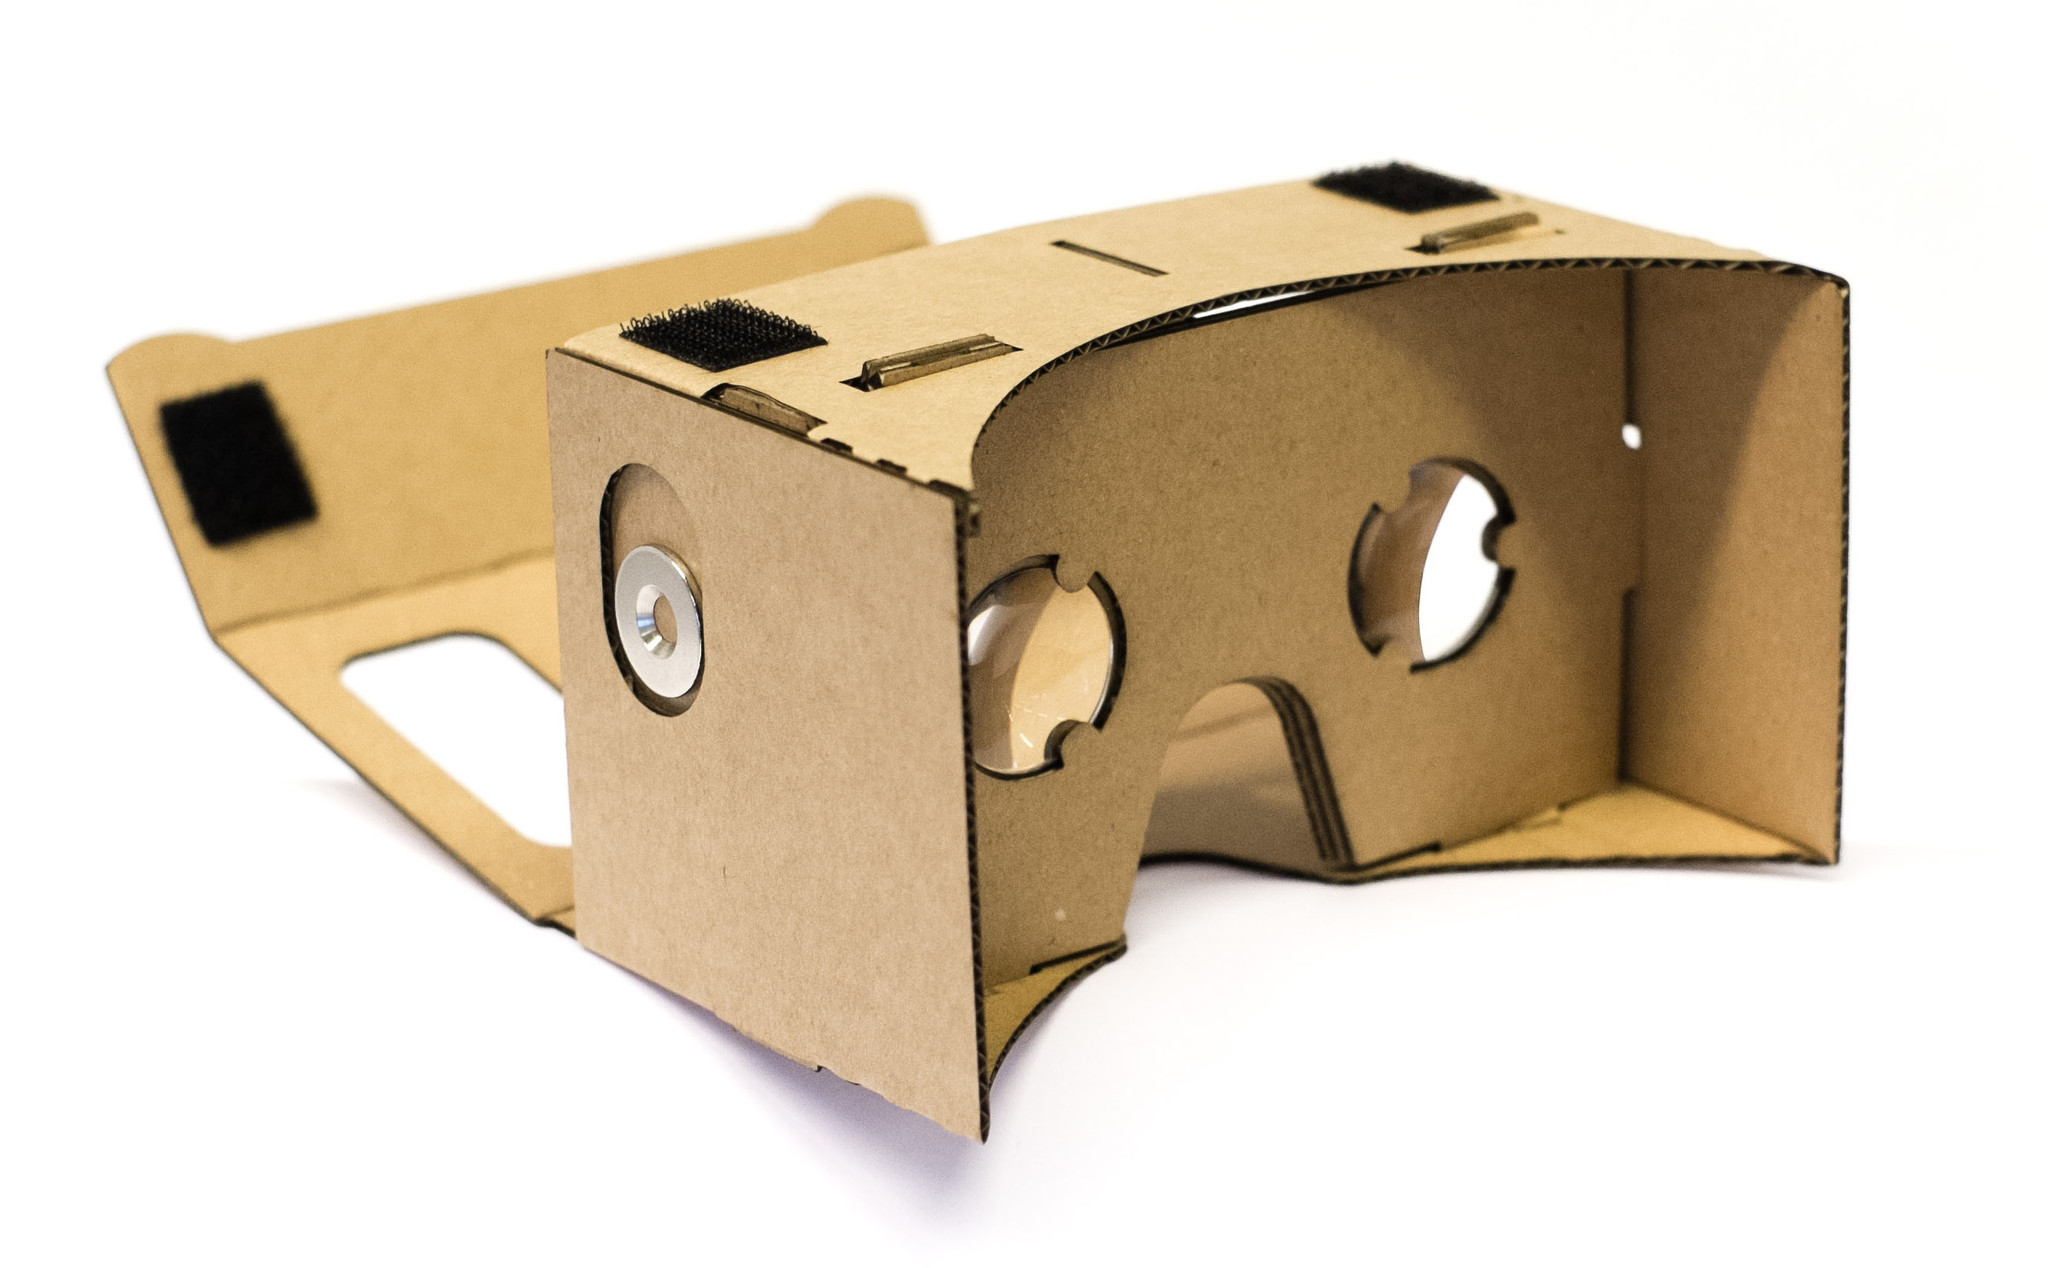
\includegraphics[width=0.4\textwidth]{res/img/cardboard2.jpg}
  \caption{Google Cardboard sans téléphone}
\end{figure}